\documentclass[a4paper,10pt]{report}
\pagestyle{plain}
\usepackage{graphicx}
\usepackage{caption}
\usepackage{algorithmic}
% Title Page
\title{Half-Wave Rectifier}
\author{Generated by SMCSim}

\begin{document}
\maketitle
\hrule\vspace{5mm}
\begin{center} {\bf Simulation of ckt/HWRectifierFilter.ckt} \end{center}
\hrule\vspace{5mm}

{\bf Circuit Diagram:} \\
\vspace{2mm}
\hrule\vspace{5mm}

{\bf NetList:} \\
{\it * Half-Wave Rectifier} \\
V1 1 0 sine (5 50) \\
D1 1 2 mymodel (1e-8 0.026) \\
R1 2 0 10000 \\
C1 2 0 10e-3 \\
.tran 0 100 0.5 \\
.plot v(1) v(2) \\
.end 
\vspace{2mm}
\hrule\vspace{5mm}

{\bf System of Equations representing the electrical circuit:}
\vspace{2mm}
\begin{equation}
     i_{V_1} + D_{1f}(v_1,v_2) = 0 
\end{equation}
\begin{equation}
     (R_1)v_2 + (C_1)\frac{dv_2}{dt} + -D_{1f}(v_1,v_2) = 0 
\end{equation}
\begin{equation}
     v_1 = V_1
\end{equation}
\vspace{2mm}
$$ D_{nf}(v_a,v_b)=Is_n(1-e^{(v_a-v_b)/vt_n})$$
 where $Is_n$=reverse saturation current and $vt_n$=threshold voltage of diode $n$\\
\hrule\vspace{5mm}

{\bf Matrix form:}\\
The system of equations $\mathbf{A}\mathbf{x}+\mathbf{D}_f(\mathbf{\widehat{x}})+\mathbf{C}(d\mathbf{x}/dt)=b$ (Symbolically)\\
Where $\mathbf{A}$, $\mathbf{D}_f$ and $\mathbf{C}$ represent matrices corresponding to linear,
  nonlinear and time dependent electrical elements respectively.
  $\mathbf{b}$ represents the vector corresponding to sources.

\begin{equation}
\mathbf{A}=  
\left[ 
\begin{array}{ccc} 
0 &0  &1  \\ 
0 &\widehat{R}_1 &0  \\ 
1 &0  &0  
\end{array}
\right]
\end{equation} 
\begin{equation}
\mathbf{b}=  
\left[ 
\begin{array}{c} 
0  \\ 
0   \\ 
V_1  
\end{array}
\right]
\end{equation} 
\begin{equation}
\mathbf{D}_f=  
\left[ 
\begin{array}{c} 
D_{1f}  \\ 
-D_{1f}   \\ 
0  
\end{array}
\right]
\end{equation} 
\begin{equation}
\mathbf{C}=  
\left[ 
\begin{array}{ccc} 
0 &0  &0  \\ 
0 &C_1 &0  \\ 
0 &0  &0  
\end{array}
\right]
\end{equation} 
\begin{equation}
\mathbf{x}=  
\left[ 
\begin{array}{c} 
v_1   \\ 
v_2    \\ 
i_{V_1}  
\end{array}
\right]
\end{equation} 
\begin{equation}
\mathbf{\widehat{x}}=  
\left[ 
\begin{array}{c} 
(v_1,v_2)     
\end{array}
\right]
\end{equation} 
Note that the matrix contains $\widehat{R}$ entries (corresponding to resistors) whose values are equal to 1/$R$\\
\hrule\vspace{2mm}
The number of equations are $3$ \\
Unknowns: \\
  Node potentials: $2$ Current Variables: $1$ \\
\hrule\vspace{5mm}

{\bf Operating Point (DC) Analysis: } \\
{\it All capacitors are open circuited and inductors are short circuited.} 
\vspace{2mm}

{\bf System of Equations representing the electrical circuit:}
\begin{equation}
     i_{V_1} + D_{1f}(v_1,v_2) = 0 
\end{equation}
\begin{equation}
     (R_1)v_2 + -D_{1f}(v_1,v_2) = 0 
\end{equation}
\begin{equation}
     v_1 = V_1
\end{equation}
\vspace{2mm}
$$ D_{nf}(v_a,v_b)=Is_n(1-e^{(v_a-v_b)/vt_n})$$
 where $Is_n$=reverse saturation current and $vt_n$=threshold voltage of diode $n$\\
\hrule\vspace{5mm}

{\bf Application of Newton-Raphson method: }\\
\vspace{2mm}
{\it Nonliner models: }\\   
See linearized model for diode $D_1$ in diode\_D1.eps
\begin{figure}[h]
\centering

\includegraphics{diode_D1.eps}
\caption{linearization of diode $D_1$}
\end{figure}
\vspace{2mm}

{\bf System of Equations representing the electrical circuit:}\\
\begin{equation}
     (R_{D_1})v_1 + (-R_{D_1})v_2 + i_{V_1} = -i_{D_1} 
\end{equation}
\begin{equation}
    (R_{D_1})v_1 + (R_{D_1}+R_1)v_2 = i_{D_1} 
\end{equation}
\begin{equation}
     v_1 = V_1
\end{equation}
\hrule\vspace{5mm}

{\bf Transient Analysis:} \\
\hrule\vspace{5mm}

{\bf Results:} \\
\begin{figure}[h]
\centering
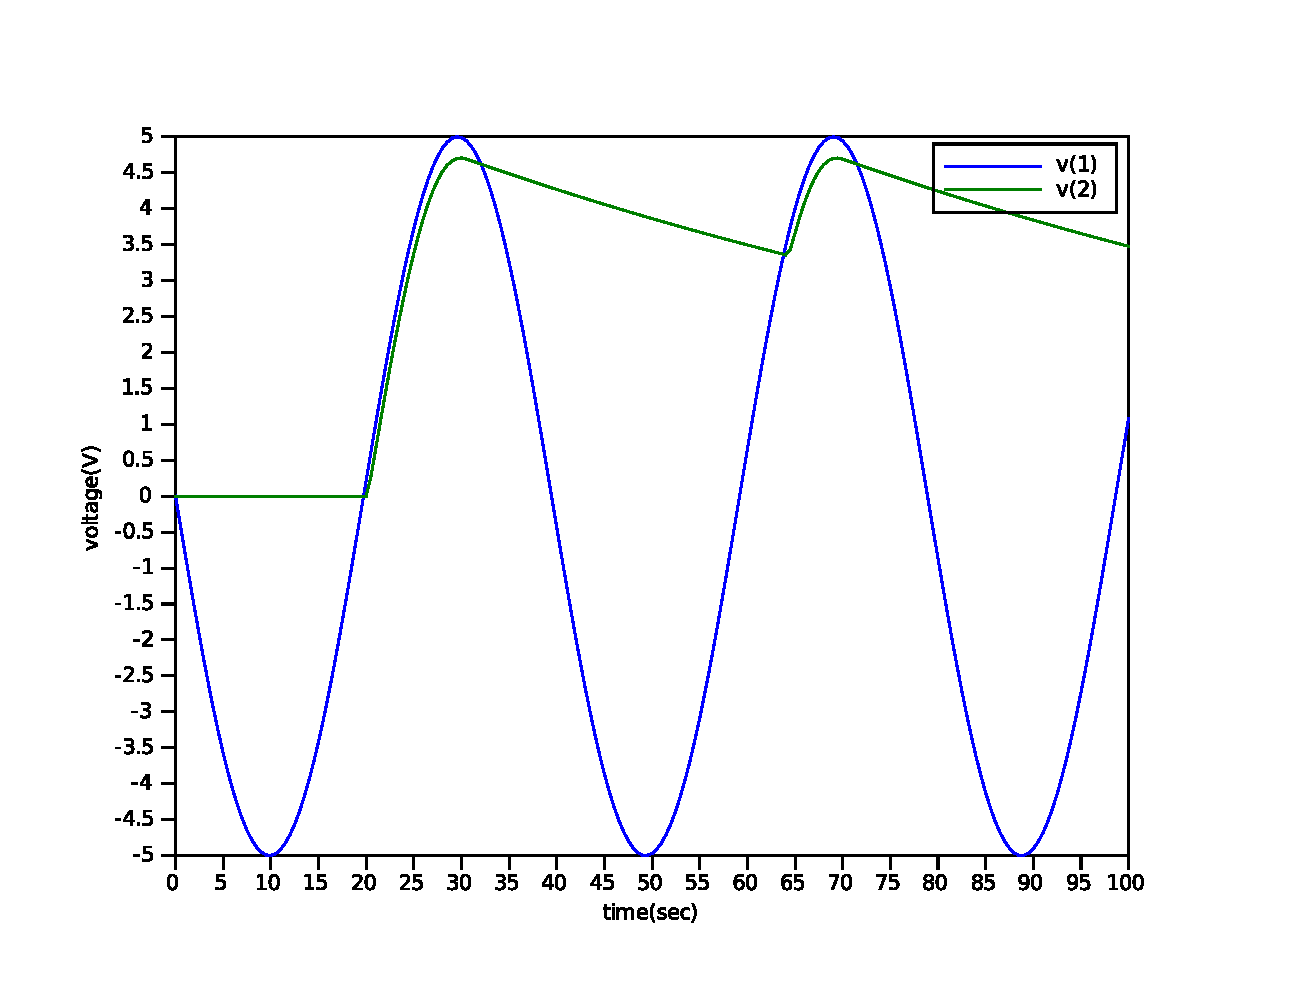
\includegraphics[scale=0.5]{output.eps}
\caption{plot}
\end{figure}


\end{document}

